\section{Lecture 3: 26.08.2025}

\subsection{Eigenvalues and Eigenvectors}

Let $A \in \mathbb{C}^{n \times n}$ be a square matrix. An \textbf{eigenvalue} $\lambda \in \mathbb{C}$ and corresponding \textbf{eigenvector} $\mathbf{v} \in \mathbb{C}^n \setminus \{\mathbf{0}\}$ satisfy:
\begin{align}
    A \mathbf{v} &= \lambda \mathbf{v} \label{eq:eigenvalue-equation}
\end{align}

For the conjugate transpose $A^H$, we have:
\begin{align}
    A^H \mathbf{w} &= \overline{\lambda} \mathbf{w} \label{eq:conjugate-eigenvalue}
\end{align}

\begin{remark}{}{}
    If $A$ is Hermitian (i.e., $A^H = A$), then all eigenvalues are real: $\lambda \in \mathbb{R}$.
    If $A$ is singular, then $\lambda = 0$ is an eigenvalue.
\end{remark}

\subsection{Matrix Properties and Non-singularity}

\begin{definition}{Strictly Diagonally Dominant Matrix}{strict-diagonal-dominant}
    A matrix $A \in \mathbb{C}^{n \times n}$ is \textbf{strictly diagonally dominant} if
    \begin{equation}
        |a_{ii}| > \sum_{\substack{j=1 \\ j \neq i}}^n |a_{ij}| \quad \text{for all } i = 1, 2, \ldots, n
    \end{equation}
\end{definition}

\begin{theorem}{Non-singularity of Strictly Diagonally Dominant Matrices}{strict-dd-nonsingular}
    Every strictly diagonally dominant matrix is non-singular.
\end{theorem}

\begin{definition}{Irreducible Matrix}{irreducible-matrix}
    A matrix $A \in \mathbb{C}^{n \times n}$ is \textbf{irreducible} if for every pair of indices $i, j \in \{1, 2, \ldots, n\}$, there exists a sequence of indices $i = m_0, m_1, m_2, \ldots, m_k = j$ such that $a_{m_\ell m_{\ell+1}} \neq 0$ for all $\ell = 0, 1, \ldots, k-1$.

    Equivalently, the directed graph associated with the matrix is strongly connected.
\end{definition}


    A matrix $A$ is \textbf{reducible} if and only if there exists a permutation matrix $P$ such that
    \begin{equation}
        P A P^T = \begin{bmatrix}
            A_{11} & A_{12} \\
            \mathbf{0} & A_{22}
        \end{bmatrix}
    \end{equation}
    where $A_{11}$ and $A_{22}$ are square matrices.

\begin{theorem}{Irreducible Diagonally Dominant Matrices}{irreducible-dd-nonsingular}
    If $A$ is irreducible and diagonally dominant with at least one row strictly diagonally dominant, then $A$ is non-singular.
\end{theorem}

\begin{example}{Finite Difference Discretization}{}
    Consider the Poisson equation $\Delta u = u_{xx} + u_{yy} = f(x, y)$ on domain $\Omega$ with boundary condition $u = g$ on $\Gamma \subset \partial \Omega$.

    The finite difference discretization yields the linear system:
    \begin{equation}
        \alpha_{pp}U_{p} + \sum_{\ell=1}^{N_p} \alpha_{pQ_\ell} U_{Q_\ell} = f_p \quad \text{for } p = 1, 2, \ldots, M
    \end{equation}
    where:
    \begin{itemize}
        \item $p$ is a grid point in the interior domain
        \item $Q_\ell$ are the neighboring points of $p$
        \item $N_p$ is the number of neighbors of $p$
        \item $U_p$ is the approximate solution at grid point $p$
    \end{itemize}

    \begin{center}
    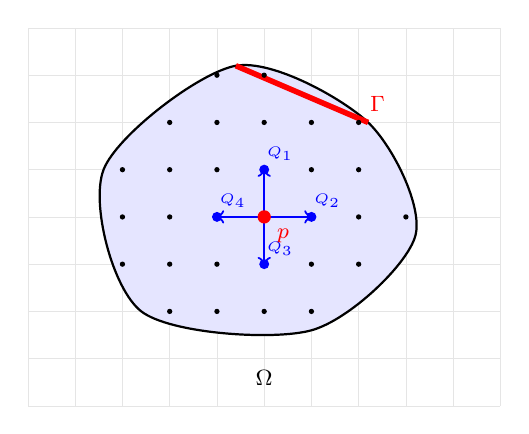
\begin{tikzpicture}[scale=1.2, every node/.style={font=\small}]
        % Domain boundary (smooth closed curve)
        \def\domcoords{(1.2,1) (3,0.8) (4.1,1.8) (3.6,3) (2.2,3.6) (0.8,2.5)}

        % Background grid
        \draw[step=0.5,very thin,gray!20] (0,0) grid (5,4);

        % Domain region
        \draw[fill=blue!10,draw=black,thick] plot[smooth cycle] coordinates \domcoords;

        % Highlight boundary segment Gamma
        \draw[line width=2pt,red] plot[smooth,tension=0.7] coordinates {(3.6,3) (2.9,3.3) (2.2,3.6)};
        \node[red,font=\footnotesize] at (3.7,3.2) {$\Gamma$};

        % Interior grid points
        \begin{scope}
            \clip plot[smooth cycle] coordinates \domcoords;
            \foreach \x in {0.5,1.0,...,4.5}{
                \foreach \y in {0.5,1.0,...,3.5}{
                    \fill[black] (\x,\y) circle (0.8pt);
                }
            }
        \end{scope}

        % Highlight central point p and neighbors
        \coordinate (p) at (2.5,2.0);
        \coordinate (Q1) at (2.5,2.5);   % north
        \coordinate (Q2) at (3.0,2.0);   % east
        \coordinate (Q3) at (2.5,1.5);   % south
        \coordinate (Q4) at (2.0,2.0);   % west

        % Draw connections
        \foreach \q in {Q1,Q2,Q3,Q4}{
            \draw[->,blue,thick] (p) -- (\q);
        }

        % Mark points
        \fill[red] (p) circle (2pt);
        \node[red,font=\footnotesize] at (2.7,1.8) {$p$};

        \foreach \i/\name in {Q1/$Q_1$,Q2/$Q_2$,Q3/$Q_3$,Q4/$Q_4$}{
            \fill[blue] (\i) circle (1.5pt);
            \node[blue,font=\tiny] at (\i) [shift={(0.2,0.2)}] {\name};
        }

        \node[font=\footnotesize] at (2.5,0.3) {$\Omega$};
    \end{tikzpicture}
    \end{center}
\end{example}

\subsection{Gershgorin Circle Theorem}

\begin{theorem}{Gershgorin Circle Theorem}{gershgorin}
    Let $A = (a_{ij}) \in \mathbb{C}^{n \times n}$ and define the \textbf{row radii}:
    \begin{equation}
        R_i = \sum_{\substack{j=1 \\ j \neq i}}^n |a_{ij}| \quad \text{for } i = 1, 2, \ldots, n
    \end{equation}

    Then every eigenvalue of $A$ lies within the union of \textbf{Gershgorin discs}:
    \begin{equation}
        \sigma(A) \subseteq S_R = \bigcup_{i=1}^n D(a_{ii}, R_i)
    \end{equation}
    where $D(a_{ii}, R_i) = \{ z \in \mathbb{C} : |z - a_{ii}| \leq R_i \}$ is the closed disc centered at $a_{ii}$ with radius $R_i$.
\end{theorem}

\begin{center}
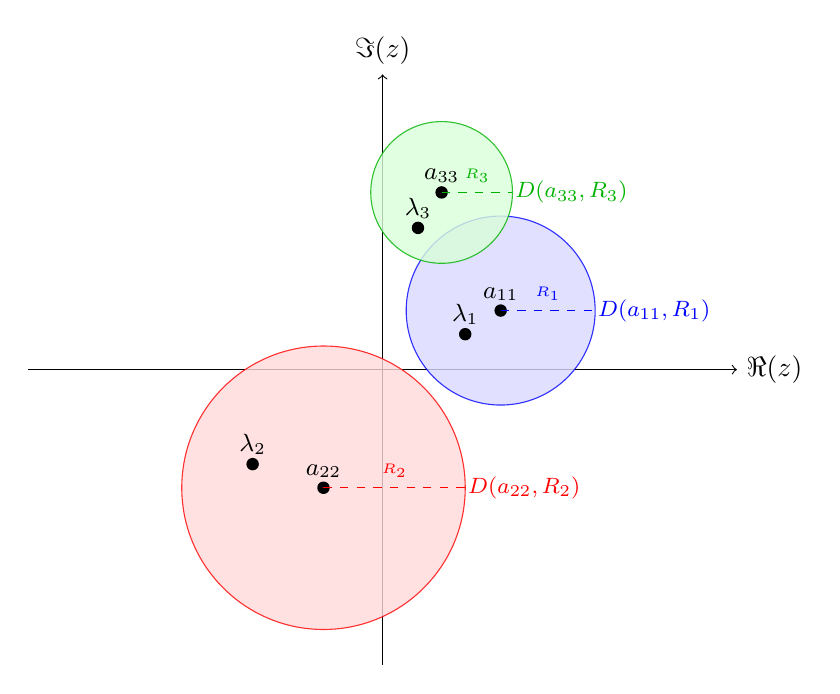
\begin{tikzpicture}[scale=1.5]
    % Complex plane axes
    \draw[->] (-3,0) -- (3,0) node[right] {$\Re(z)$};
    \draw[->] (0,-2.5) -- (0,2.5) node[above] {$\Im(z)$};

    % Diagonal elements
    \coordinate (a11) at (1,0.5);
    \coordinate (a22) at (-0.5,-1);
    \coordinate (a33) at (0.5,1.5);

    % Gershgorin discs
    \draw[blue, fill=blue!15, opacity=0.8] (a11) circle (0.8);
    \draw[red, fill=red!15, opacity=0.8] (a22) circle (1.2);
    \draw[green!70!black, fill=green!15, opacity=0.8] (a33) circle (0.6);

    % Diagonal elements
    \fill[black] (a11) circle (1.5pt) node[above, font=\small] {$a_{11}$};
    \fill[black] (a22) circle (1.5pt) node[above, font=\small] {$a_{22}$};
    \fill[black] (a33) circle (1.5pt) node[above, font=\small] {$a_{33}$};

    % Sample eigenvalues
    \fill[black] (0.7,0.3) circle (1.5pt) node[above, font=\small] {$\lambda_1$};
    \fill[black] (-1.1,-0.8) circle (1.5pt) node[above, font=\small] {$\lambda_2$};
    \fill[black] (0.3,1.2) circle (1.5pt) node[above, font=\small] {$\lambda_3$};

    % Disc labels
    \node[blue, font=\footnotesize] at (2.3,0.5) {$D(a_{11}, R_1)$};
    \node[red, font=\footnotesize] at (1.2,-1) {$D(a_{22}, R_2)$};
    \node[green!70!black, font=\footnotesize] at (1.6,1.5) {$D(a_{33}, R_3)$};

    % Radius indicators
    \draw[blue, dashed] (a11) -- ++(0.8,0) node[midway, above, font=\tiny] {$R_1$};
    \draw[red, dashed] (a22) -- ++(1.2,0) node[midway, above, font=\tiny] {$R_2$};
    \draw[green!70!black, dashed] (a33) -- ++(0.6,0) node[midway, above, font=\tiny] {$R_3$};
\end{tikzpicture}
\end{center}

\begin{theorem}{Gershgorin Separation}{gershgorin-separation}
    Let $S_1 = \bigcup_{i=1}^\ell D(a_{ii}, R_i)$ and $S_2 = \bigcup_{i=\ell+1}^n D(a_{ii}, R_i)$ where $S_1 \cap S_2 = \emptyset$.

    Then $A$ has exactly $\ell$ eigenvalues in $S_1$ and $n-\ell$ eigenvalues in $S_2$.
\end{theorem}

\begin{theorem}{Gershgorin for Irreducible Matrices}{gershgorin-irreducible}
    If $A$ is irreducible and $\lambda$ lies on the boundary of some Gershgorin disc $\partial D(a_{ii}, R_i)$, then $\lambda$ lies on the boundary of every Gershgorin disc.
\end{theorem}

\begin{proof}[Proof of Theorem~\ref{thm:gershgorin}]
    Let $\lambda \in \sigma(A)$ with corresponding eigenvector $\mathbf{v} = (v_1, v_2, \ldots, v_n)^T$.
    Normalize so that $\|\mathbf{v}\|_\infty = 1$, and let $m$ be an index such that $|v_m| = 1$.

    From the eigenvalue equation $A\mathbf{v} = \lambda\mathbf{v}$, the $m$-th component gives:
    \begin{align}
        \sum_{j=1}^n a_{mj} v_j &= \lambda v_m \\
        (\lambda - a_{mm}) v_m &= \sum_{\substack{j=1 \\ j \neq m}}^n a_{mj} v_j
    \end{align}

    Taking absolute values and using $|v_j| \leq 1$ for all $j$:
    \begin{align}
        |\lambda - a_{mm}||v_m| &= \left|\sum_{\substack{j=1 \\ j \neq m}}^n a_{mj} v_j\right| \\
        &\leq \sum_{\substack{j=1 \\ j \neq m}}^n |a_{mj}||v_j| \\
        &\leq \sum_{\substack{j=1 \\ j \neq m}}^n |a_{mj}| = R_m
    \end{align}

    Since $|v_m| = 1$, we have $|\lambda - a_{mm}| \leq R_m$, so $\lambda \in D(a_{mm}, R_m) \subseteq S_R$.
\end{proof}

\begin{proof}[Proof of Theorem~\ref{thm:gershgorin-irreducible}]

    Suppose $\lambda$ lies on the boundary of $D(a_{mm}, R_m)$. Then equality holds in the previous proof:
    \begin{equation}
        |\lambda - a_{mm}| = \sum_{\substack{j=1 \\ j \neq m}}^n |a_{mj}|\frac{|v_j|}{|v_m|} = R_m
    \end{equation}

    This requires $|v_j| = |v_m|$ for all $j$ such that $a_{mj} \neq 0$.

    Since $A$ is irreducible, for any indices $i, j$, there exists a path $i = m_0, m_1, \ldots, m_k = j$ with $a_{m_\ell m_{\ell+1}} \neq 0$ for all $\ell = 0, 1, \ldots, k-1$.

    By the same argument, we get $|v_{m_\ell}| = |v_{m_{\ell+1}}|$ for all $\ell$, which implies $|v_i| = |v_j|$ for all $i, j$.

    Therefore, $|\lambda - a_{ii}| = R_i$ for all $i$, meaning $\lambda$ lies on the boundary of every Gershgorin disc.
\end{proof}

\subsection{Continuity of Eigenvalues}

Consider the matrix family $A(t) = D + tH$ where $D$ is diagonal and $H$ contains the off-diagonal entries of $A$, with $t \in [0,1]$.

\begin{align}
    A(t) &= D + tH \quad \text{where} \begin{cases}
        A(0) = D & \text{(diagonal matrix)} \\
        A(1) = A & \text{(original matrix)}
    \end{cases}
\end{align}

The eigenvalues $\lambda(t)$ of $A(t)$ vary continuously with respect to $t$. The eigenvalues of $A(0) = D$ are simply $a_{11}, a_{22}, \ldots, a_{nn}$.

If $D$ has distinct diagonal entries, then as $t$ varies from 0 to 1, each eigenvalue remains within its corresponding Gershgorin disc, providing insight into eigenvalue perturbation.